\subsection{Versão 3 - Reimplementação para interpretação do MEC em 2017 }
\label{versao3}

Com objetivo de unificar o entendimento da distribuição de cotas, o \gls{MEC} lançou em seu portal as alterações e detalhes sobre como deveria ser implementada a nova regra de ingresso em vestibulares e processos seletivos da rede federal. Na Figura \ref{fig:mec}, pode-se observar a nova divisão, que agora abrange \gls{PPI} que possuam alguma deficiência e \gls{PPI} que não possuam deficiência, tanto para os estudantes de escolas públicas com renda inferior, como estudantes de renda superior a 1,5 salários mínimos. 

\begin{figure}[ht!]
\centering

\caption{\textmd{Novo procedimento de aplicação do sistema de cotas}}
\label{fig:mec}
\fcolorbox{gray}{white}{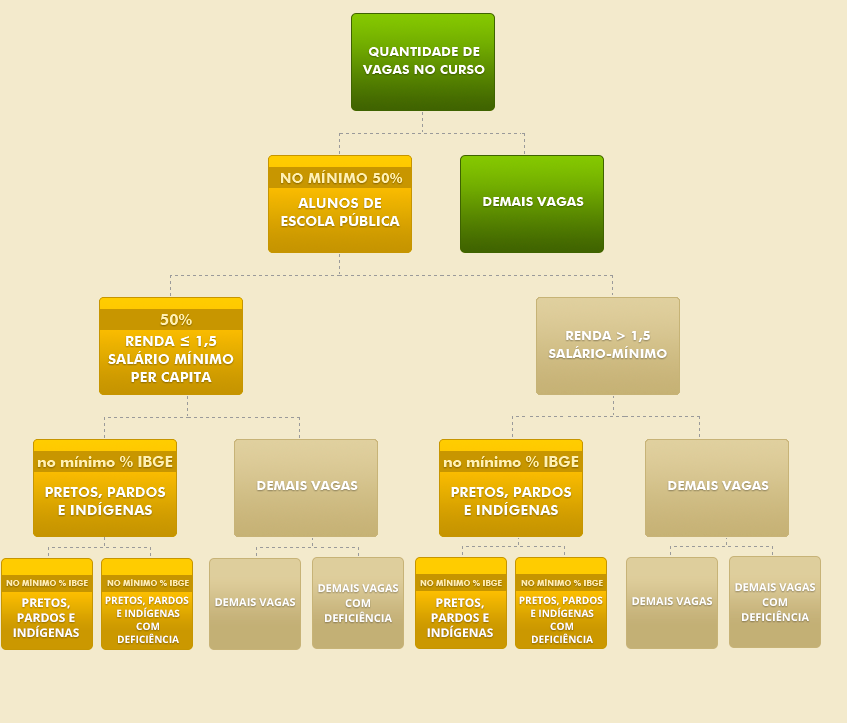
\includegraphics[width=0.67\textwidth]{chapters/sistemaingresso_versoes/imagens/mec.png}}

\par\medskip\textbf{Fonte:} \citeonline{sitemec}. \par\medskip

\end{figure}




Na versão anterior da implementação, o aluno teria que optar por concorrer entre as opções: \gls{PPI}, somente \gls{PCD} ou nas demais vagas, causando problemas durante as inscrições de várias instituições de ensino, pois haviam candidatos que eram tanto \gls{PPI} como \gls{PCD} e tinham direito a concorrer nas duas categorias de cota.

Tendo em vista a correção do entendimento feita pelo \gls{MEC}, foi preciso criar 9 (nove) tipos de situações de classificação para cada combinação de cotas possível (Tabela \ref{tabela_cotasv3}).

\begin{table}[ht]
\caption{Lista de categorias de cotas da versão 3}
\label{tabela_cotasv3}
\centering
\resizebox{\textwidth}{!}{
\begin{tabular}{ l l }
   \cline{1-1}\cline{2-2}  
    \multicolumn{1}{|p{5.850cm}|}{\textbf{CLAG}} &
    \multicolumn{1}{p{8.217cm}|}{Ampla concorrência ou classificação geral}
  \\ 
   \cline{1-1}\cline{2-2}  
    \multicolumn{1}{|p{5.850cm}|}{\textbf{RIPPIPCDR1}} &
    \multicolumn{1}{p{8.217cm}|}{Renda igual ou inferior a 1,5 (um vírgula cinco) salário-mínimo per capita autodeclarados pretos, pardos ou indígenas com deficiência (PcD PPI).}
  \\    
   \cline{1-1}\cline{2-2}  
    \multicolumn{1}{|p{5.850cm}|}{\textbf{RINPPIPCDR2}} &
    \multicolumn{1}{p{8.217cm}|}{Estudante de escolas públicas brasileiras com renda igual ou inferior a 1,5 (um vírgula cinco) salário-mínimo per capita não autodeclarados pretos, pardos ou indígenas com deficiência (PcD Não PPI)}
  \\
   \cline{1-1}\cline{2-2}  
    \multicolumn{1}{|p{5.850cm}|}{\textbf{RSPPIPCDR3}} &
    \multicolumn{1}{p{8.217cm}|}{
Renda superior a 1,5 (um vírgula cinco) salário-mínimo per capita autodeclarados pretos, pardos, indígenas com deficiência (PcD PPI)}
  \\
  \cline{1-1}\cline{2-2}  
    \multicolumn{1}{|p{5.850cm}|}{\textbf{RSNPPIPCDR4}} &
    \multicolumn{1}{p{8.217cm}|}{
Renda superior a 1,5 (um vírgula cinco) salário-mínimo per capita não autodeclarados pretos, pardos ou indígenas com deficiência (PcD Não PPI)}
  \\
   \cline{1-1}\cline{2-2}  
    \multicolumn{1}{|p{5.850cm}|}{\textbf{RIPPIR5}} &
    \multicolumn{1}{p{8.217cm}|}{
Renda inferior a 1,5 (um vírgula cinco) salário-mínimo per capita autodeclarados pretos, pardos ou indígenas (PPI)}
 \\
   \cline{1-1}\cline{2-2}  
    \multicolumn{1}{|p{5.850cm}|}{\textbf{RINPPIR6}} &
    \multicolumn{1}{p{8.217cm}|}{
Renda inferior a 1,5 (um vírgula cinco) salário-mínimo per capita não autodeclarados pretos, pardos ou indígenas (Não PPI)
}
  \\  
   \cline{1-1}\cline{2-2}  
    \multicolumn{1}{|p{5.850cm}|}{\textbf{RSPPIR7}} &
    \multicolumn{1}{p{8.217cm}|}{
Renda superior a 1,5 (um vírgula cinco) salário-mínimo per capita autodeclarados pretos, pardos ou indígenas (PPI)
}
  \\  
   \cline{1-1}\cline{2-2}  
    \multicolumn{1}{|p{5.850cm}|}{\textbf{RSNPPIR8}} &
    \multicolumn{1}{p{8.217cm}|}{
Renda superior a 1,5 (um vírgula cinco) salário-mínimo per capita não autodeclarados pretos, pardos ou indígenas (Não PPI)
}
  \\   
  \hline

 \end{tabular}}
\end{table}


Tendo como base essas novas categorias, a Figura \ref{fig:cenario3} detalha o terceiro cenário de classificação para um curso de 40 vagas. 

\begin{figure}[ht!]
\centering

\caption{\textmd{Cenário de distribuição versão 3}}
\label{fig:cenario3}
\fcolorbox{gray}{white}{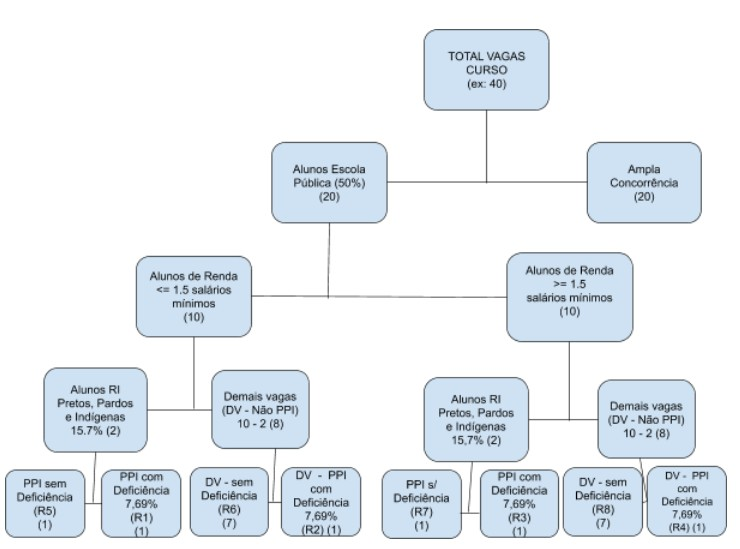
\includegraphics[width=0.9\textwidth]{chapters/sistemaingresso_versoes/cenarios/cenario3.jpg}}

\par\medskip\textbf{Fonte:} Elaborada pelo autor (2019). \par\medskip
\end{figure}



\newpage
Diante da crescente demanda por alterações nas funções de classificação por cotas, a \gls{DTIC} optou por refatorar o código de modo que as regras de distribuição não fossem implementadas de forma estática no código fonte, esta versão foi implementada com armazenamento da árvore de cotas em banco de dados, como uma tentativa de diminuir o impacto em novas mudanças por parte dos desenvolvedores. 

Nesta versão houve uma redução de linhas de código considerável e a equipe centralizou rotinas responsáveis pelos cálculos em apenas um arquivo \texttt{calculo\_cotas.php}. Nesse arquivo foram criadas as funções, \texttt{obtem\_arvore\_cotas} e \texttt{calcula\_cotas} (Código Fonte \ref{lst:arvorecotas}), que fazem a consulta de configurações e percentuais necessários para o cálculo do quadro de vagas. 

As novas funções foram importadas em todos os arquivos envolvidos nos processos de classificação de candidatos, e as funções antigas precisaram ser alteradas para buscar as configurações de cotas de maneira dinâmica, como pode ser visto no Código Fonte \ref{lst:novafuncaoprioridade}, que agora busca a ordem de prioridade de sobra de vagas da base de dados. 

\lstinputlisting[language=PHP, 
caption=Nova funções quadro de vagas
,label=lst:arvorecotas]{chapters/trechos_codigo/arvorecotas.m}

\lstinputlisting[language=PHP, 
caption=Nova função de prioridade para sobra de vagas
,label=lst:novafuncaoprioridade]{chapters/trechos_codigo/funcoescatdinamicas.m}

Embora a inclusão das configurações de cotas no banco de dados tenha ajudado na redução de código fonte estático a ser modificado, ainda surgiram novas demandas de ajustes para determinados tipos de processos nos quais a área demandante precisou da intervenção da equipe de desenvolvimento. Estas situações são
exemplificadas na Seção \ref{outrasVersoes}.